\documentclass{article}

\usepackage{graphicx}

\author{Ee Xuan Tan (4907531) \and Elvira Voorneveld (4930975) \and William Narchi (5046122)}
\date{Group 40} % A small hack to add the group number AND get rid of the date
\title{Computer Graphics Project}

\begin{document}
    \maketitle

    \section{Work Distribution}
    To be constructed

    \section{Features}
    \subsection{Main Requirements}
    \subsubsection{Recursive Ray Tracing}
    The recursive ray tracer builds upon the previously implemented ray shading,
    creating reflection rays at each intersection point and adding the value of the reflection ray's lighting to the initial ray's specular component,
    provided that the intersection point is on a specular surface and that the reflected ray interesects a surface.
    This is done recursively until one of the previously mentioned limiting conditions applies or the recursion depth reaches a pre-set \emph{RECURSION\_LIMT}.

    \begin{center}
        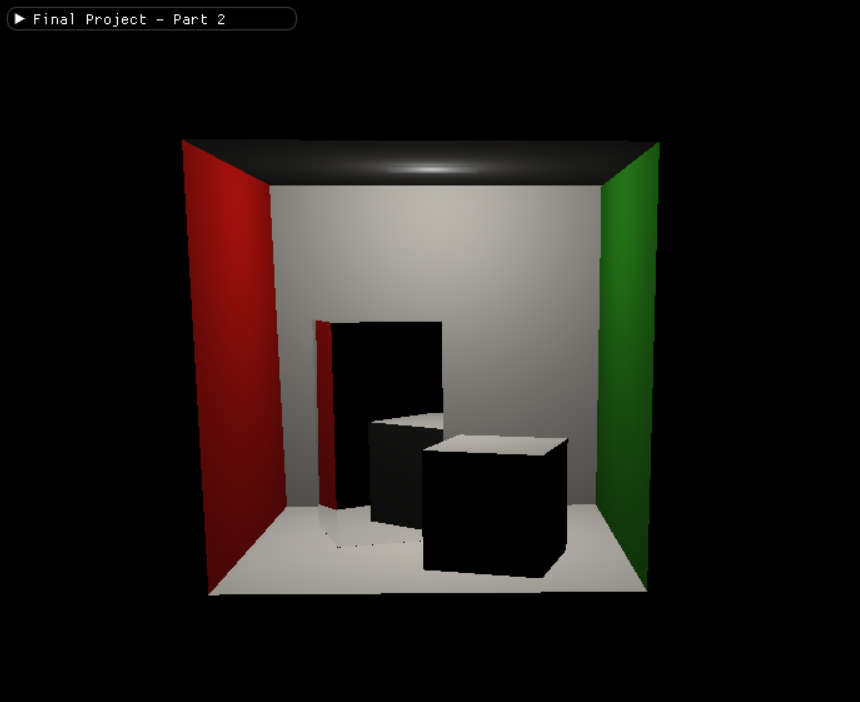
\includegraphics[scale=0.70]{images/recursive_ray_tracer_showcase.png}

        The complex specular effects produced by recursive ray tracing, which include proper mirror simulation

        \vspace{5mm}

        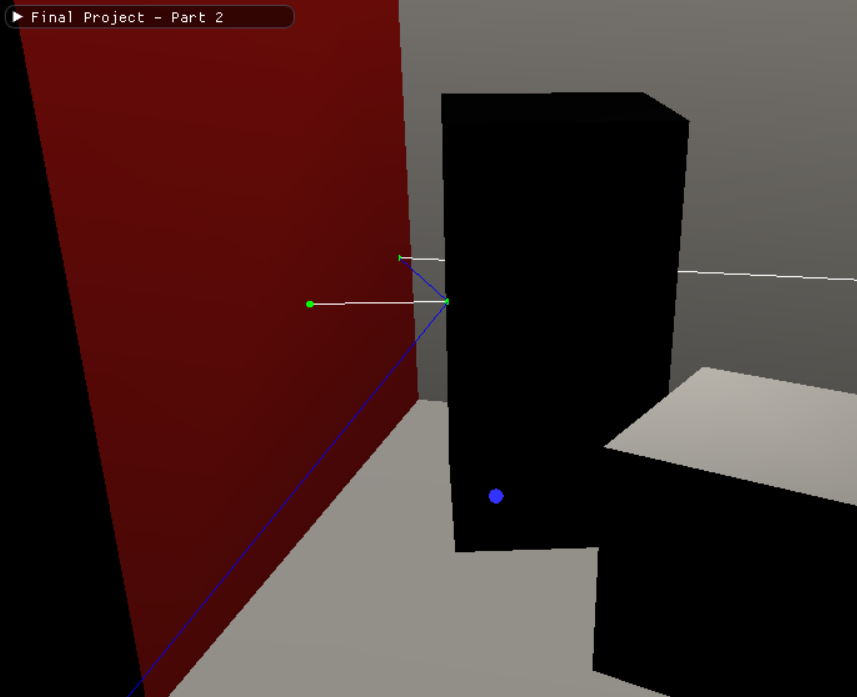
\includegraphics[scale=0.70]{images/recursive_ray_tracer_debug.png}

        The recursive ray tracer debug, showing two total rays in the recursive chain, along with their normals
    \end{center}
    \subsubsection{Soft Shadows}
    The first step to the implementing the soft shadows is to generate uniformly distributed rays from the spherical light source. 
    In order, to get a uniform distribution of rays from the lightsource, the idea of the fibonacci sequence was used, by generating unifromly distributed 
    step sizes using the golden ratio. The second problem, was to remove light rays
    from the 'wrong' side of the light source, this was done by using the center of the sphere and radius to calculate the longest the light ray on the 'right' side could be.
    So, by using this method we are able to check each randomly generated sample of the light. Finally, a number of sample points are taken, from these sample points we check to see if they are on the 'right' side of the sphere
    and if the sample ray does not intersect an object. For each point we then divide the lighting value obtained by the number of sample rays taken from the sphere, giving the average light value. 

    \begin{center}
        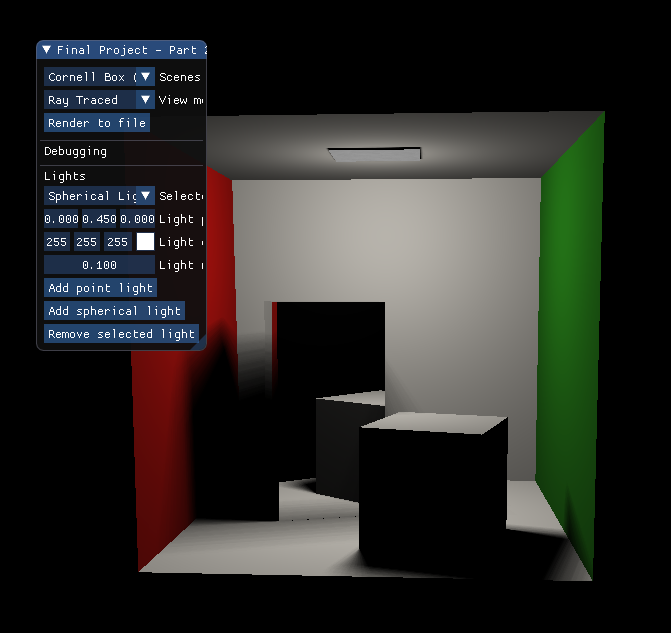
\includegraphics[scale=0.70]{images/softshadow_showcase.png}

        The soft shadow result when SPHERE SAMPLE LIMIT has been set to 100 samples.

        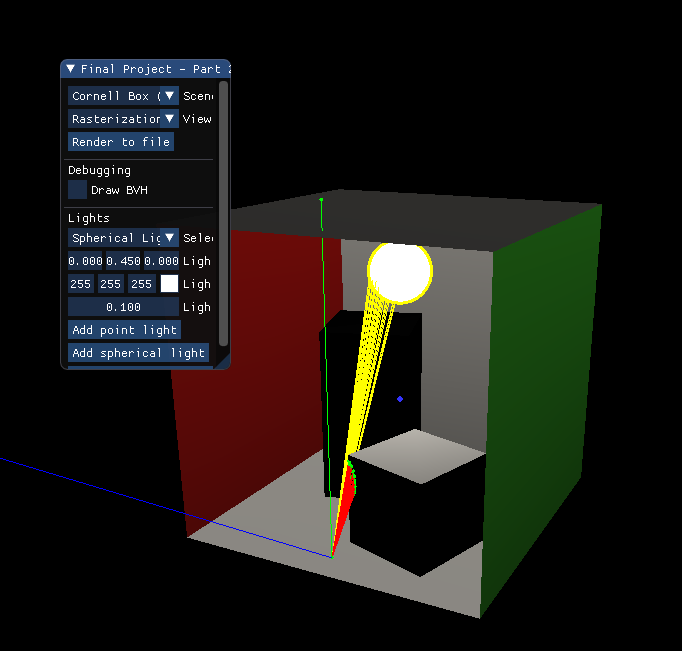
\includegraphics[scale=0.70]{images/softshadowdebug.png}

        The soft shadow debug, showing random samples generated uniformly from the spherical lightsource and showcasing the rays that intersect an objects and those that do not.  

    \end{center}

    \section{Models}
    To be constructed

    \section{Performance Test}
    To be constructed
\end{document}
